\documentclass[a4paper,11pt]{article}

\usepackage[T1]{fontenc}
\usepackage[polish]{babel}
\usepackage[utf8]{inputenc}
\usepackage{lmodern}
\selectlanguage{polish}
\usepackage[top=2cm, bottom=2cm, left=3cm, right=3cm]{geometry}
\makeatletter
\newcommand{\linia}{\rule{\linewidth}{0.4mm}}
\renewcommand{\maketitle}{\begin{titlepage}
    \vspace*{2cm}
    \begin{center}\LARGE
    Politechnika Warszawska\\
    Wydział Elektryczny\\
    \end{center}
    \vspace{5cm}
    \noindent\linia
    \begin{center}
      \LARGE \textsc{\@title}
         \end{center}
     \linia
    \vspace{0.5cm}
    \begin{flushright}
    \begin{minipage}{5cm}
    \textit{Autorzy:}\\
    \normalsize \textsc{\@author} \par
    \end{minipage}
    \vspace{5cm}
     \end{flushright}
    \vspace*{\stretch{6}}
    \begin{center}
    \@date
    \end{center}
  \end{titlepage}%
}
\makeatother
\author{Grzegorz Kopyt\\
Daniel Sporysz}
\title{Specyfikacja Funkcjonalna \\
"Automat Komórkowy"}
\usepackage{graphicx}

\begin{document}

\maketitle


\tableofcontents
\vspace{1cm}
\noindent\linia
\section{Opis działania}
Program jest implementacją automatu komórkowego opartego na regułach "gry w życie" Johna Conwaya w wariancie ,,WireWorld".

Praca programu polega na animacji obrazu wprowadzonego przez użytkownika lub wykreowanego w jednym z dwóch edytorów programu. Na jego podstawie program tworzy kolejne generacje obrazu, zgodnie z regułami "WireWorld".

Wynik działania programu jest prezentowany w oknie dialogowym, w formie animacji. Prezentacja może zostać przez użytkownika wstrzymana, edytowana lub przywrócona do stanu początkowego.

\noindent\linia
\section{Funkcje}
Program oferuje następujące funkcje:
\begin{itemize}
\item Załadowanie planszy z pliku png
\item Kontrola nad przebiegiem animacji: pauzowanie, uruchamianie, powrót do początkowej konfiguracji
\item Własnoręczna edycja planszy w trakcie pracy programu.
\item Wstawiane obiektów z przygotowanej biblioteki obiektów WireWorld
\end{itemize}



\noindent\linia
\section{Obsługa}
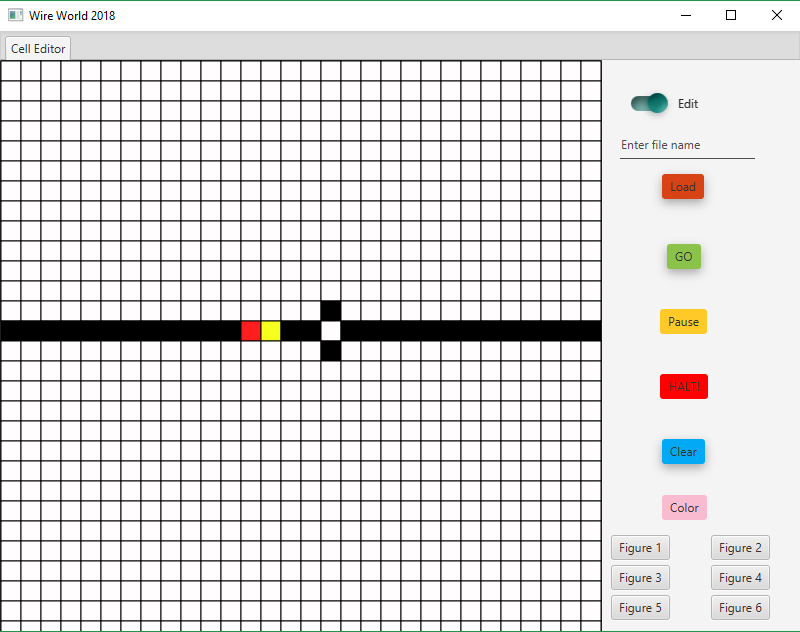
\includegraphics[width=\textwidth]{GUI_WireWorld}


\noindent\linia
\section{Sytuacje wyjątkowe}



\end{document}



